\documentclass{article}
\usepackage[utf8]{inputenc}
\usepackage{url}
\usepackage{graphicx}
\usepackage{amsmath}
\graphicspath{ {./} }


\title{Prédiction de l'âge à partir de photographies}
\date{État de l'art}

\begin{document}

\maketitle

\section{Introduction}
Pour faire une prédiction de l'âge, diverses méthodes en deep learning existent.
\begin{itemize}
    \item La classification multi classes
    \item La régression
    \item La classification ordonnée
\end{itemize}
Nous allons rapidement faire le tour des méthodes existantes. Mais d'abord, un rappel de ce qu'il y aura en commun :
\begin{itemize}
    \item Pour évaluer le modèle, on utilise mean absolute error : $MAE = \frac{\sum^{N}_{i=1}|prédit_{i}-connu_{i}|}{N}$
    \item Plus MAE est faible, plus le modèle est précis.
\end{itemize}

\section{DEX: Deep EXpectation of Apparent Age from a Single Image}
\url{https://openaccess.thecvf.com/content_iccv_2015_workshops/w11/papers/Rothe_DEX_Deep_EXpectation_ICCV_2015_paper.pdf}
DEX s'appuie sur plusieurs choses :
\begin{itemize}
    \item Un plus grand dataset (IMDB wiki), qui nous est donc pas très utile ici.
    \item Expected value : une méthode pour affiner légèrement les résultats.
    \item Une classification multiclasse classique autrement, avec softmax, crossentropy.
    \item Introduction d'une autre métrique utile d'après les auteurs car "Note that the error (MAE) does not capture the uncertainty in the ground truth labeled age. The $\epsilon$-error covers such aspect.": $\epsilon = 1-e^{\frac{(x-\mu)^2}{2\sigma^2}}$
    
\end{itemize}

\section{Age and Gender Prediction using Deep CNNs and Transfer Learning}
\url{https://arxiv.org/pdf/2110.12633.pdf}

\begin{itemize}
    \item À la fois prédiction par régression (continu) et classification (discrète).
    \item Pour la régression : premiers tests avec un réseau créé de zéro
    \item SENet50 entrainé sur VGGFace (FaceNet)
    \item Mean square error en fonction de loss (mais bien MAE pour l'évaluation finale) : $MSE = \frac{\sum^{N}_{i=1}(prédit_{i}-connu_{i})^2}{N}$
\end{itemize}

\section{Using Ranking-CNN for Age Estimation}
\url{https://openaccess.thecvf.com/content_cvpr_2017/papers/Chen_Using_Ranking-CNN_for_CVPR_2017_paper.pdf} \\

Cette méthode ressemble à la méthode de classification ordonnée par one-hot encoding. Le principe est de faire une classification binaire sur chaque tranche d'âge puis d'agréger le résultat pour avoir finalement une sortie discrète (une classe) correspondant à un âge. L'intuition derrière cette méthode est qu'il est plus simple de prédire si une personne est plus ou moins agé qu'une autre que de prédire directement son âge.

\section{Diagnosing deep learning models for high accuracy age estimation from a single image}
\url{https://www.sciencedirect.com/science/article/abs/pii/S0031320317300079}

Ce papier introduit deux nouvelles métriques pour évaluer la précision du modèle, cumulative correct score :
\begin{equation}
    CCS(t) = \sum^{N}_{i=1}h(|prédit_{i}-connu_{i}|-t)
\end{equation}
\begin{equation}
    h(x) =
    \begin{cases}
      1 & \text{if bank $x \le 0$}\\
      0 & \text{otherwise}
    \end{cases}
\end{equation}
ainsi que relative cumulative correct score : $RCCS^a_b(t) = CCA^a(t) - CCA^b(t)$ \\

D'après leurs résultats, la régression avec la métrique MAE est la plus performante de toutes les méthodes. Par ailleurs, la prédiction en parallèle de l'âge ainsi que d'autres éléments comme le sexe permet d'avoir d'encore meilleurs résultats.
\begin{figure}
    \centering
    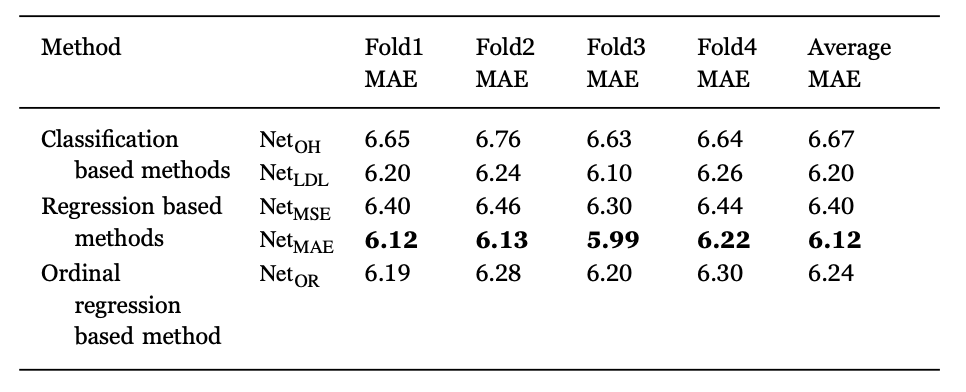
\includegraphics[width=345pt]{imgs/qualité/bibliothèque/result.png}
    \caption{Résultats obtenus par Junliang Xing, Kai Li, Weiming Hu, Chunfeng Yuan, Haibin Ling. Ce tableau montre que sur le même dataset, la méthode par régression avec la métrique mean absolute error (MAE) obtient le score le plus performant, suivi de la méthode par classification ordinal.}
    \label{fig:my_label}
\end{figure}


\section{Conclusion}

Parmis les différentes méthodes pour prédire l'âge avec le deep learning,
\begin{itemize}
    \item Réduire le problème à une classification par classe semble donner de bons résultats dans tous les cas. Il faut cependant choisir les tranches d'âges correctement, car le développement d'un mandrill n'est pas linéaire avec l'âge visuellement.
    \item La régression offre la meilleur performance si on s'en réfère aux multiples comparaisons qui figurent dans ces papiers.
    \item De manière générale, MAE est la métrique d'évaluation, et peut être également pour la fonction de coût, à retenir.
\end{itemize}

\end{document}
